%&pdflatex
%
%  Clawpack 5.x (x <= 3) Paper
%
\documentclass[]{article}

\usepackage{graphicx}
\usepackage[colorinlistoftodos]{todonotes}

% Use utf-8 encoding for foreign characters
\usepackage[utf8]{inputenc}

% Multipart figures
% \usepackage{subcaption}

% More symbols
\usepackage{amsmath}
\usepackage{amssymb}
\usepackage{latexsym}

% Package for including code in the document
\usepackage{listings}
% \DeclareCaptionFont{white}{\color{white}}
% \DeclareCaptionFormat{listing}{%
%   \parbox{\textwidth}{\colorbox{gray}{\parbox{\textwidth}{#1#2#3}}\vskip-4pt}}
% \captionsetup[lstlisting]{format=listing,labelfont=white,textfont=white}
% \lstset{frame=lrb,xleftmargin=\fboxsep,xrightmargin=-\fboxsep,numbers=left,basicstyle=\ttfamily\small,language=python,columns=fixed,commentstyle=\em\color[rgb]{0.133,0.545,0.133}}

% This is now the recommended way for checking for PDFLaTeX:
\usepackage{ifpdf}

% Add line numbers
\usepackage[mathlines]{lineno}

% Need to use this package to handle the spacing issues in LaTeX after a command
\usepackage{xspace}

% Markup
\usepackage{color}
\newcommand{\comment}[1]{{\color{blue}#1}}
\newcommand{\alert}[1]{\textbf{\color{red} #1}}

% URL and linking help with subtle colors and no boxes
\definecolor{darkgreen}{rgb}{0.1,0.5,0.1}
\definecolor{darkblue}{rgb}{0.2,0.2,1.0}
\usepackage[colorlinks=true,linkcolor=darkblue,citecolor=darkblue,
            filecolor=darkblue,urlcolor=darkgreen]{hyperref}


% Need this package to allow footnotes for more than 9 authors:
\usepackage{footmisc}

%=================
% Try using cleveref...

\usepackage[capitalize,nameinlink]{cleveref}

\crefformat{equation}{#2(#1)#3}
\crefrangeformat{equation}{(#3#1#4--#5#2#6)}
\crefmultiformat{equation}{#2(#1)#3}{ and #2(#1)#3}
{, #2(#1)#3}{, and #2(#1)#3}
\crefrangemultiformat{equation}{(#3#1#4--#5#2#6)}%
{ and (#3#1#4--#5#2#6)}{, (#3#1#4--#5#2#6)}{, and (#3#1#4--#5#2#6)}

%=================


\graphicspath{{./figures/}}


\setlength{\textwidth}{6.2in}
\setlength{\oddsidemargin}{0in}
\setlength{\evensidemargin}{0in}
\setlength{\textheight}{8.7in}
\setlength{\voffset}{-.7in}
\setlength{\headsep}{26pt}


% Useful commands
%!TEX root = paper.tex
%  Generic math macros
\renewcommand{\v}[1]{\boldsymbol{#1}}
\newcommand{\m}[1]{\text{\textsf#1}}

\newcommand{\pd}[2]{\ensuremath{\frac{\partial #1}{\partial #2}}} % partial
\newcommand{\dee}{\ensuremath{\mathrm{d}}}                  % d symbol
\newcommand{\diff}[2]{\ensuremath{\frac{\dee #1}{\dee #2}}} % Derivative d/dx
% \newcommand{\grad}{\ensuremath{\nabla}}                     % Gradient symbol
\newcommand{\gradient}{\ensuremath{\textsf{grad}}}          % Written gradient
\newcommand{\Div}{\ensuremath{\nabla \cdot}}                % Divergence
\newcommand{\divergence}{\ensuremath{\textsf{div}}}         % Written div
\newcommand{\del}{\ensuremath{\nabla}}                      % Same as gradient
\newcommand{\delsq}{\ensuremath{\nabla^2}}                  % Laplacian
\newcommand{\lap}{\ensuremath{\delsq}}                      % Laplacian
\newcommand{\dx}{\ensuremath{\Delta x}}                     % Delta x
\newcommand{\dy}{\ensuremath{\Delta y}}                     % Delta y
\newcommand{\dt}{\ensuremath{\Delta t}}                     % Delta t
\newcommand{\scinot}[2]{\ensuremath{#1\times10^{#2}}}       % Scientific note
\newcommand{\bigO}[1]{\ensuremath{\mathcal{O}(#1)}}         % Big O notation
\newcommand{\R}{\ensuremath{\mathbb{R}}}                    % Real field
\newcommand{\Z}{\ensuremath{\mathbb{Z}}}                    % Integer field
\newcommand{\half}{\ensuremath{\frac{1}{2}}}                % 1/2 fraction

%  Special formatting for codes
\newcommand{\geoclaw}{{\sc GeoClaw}\xspace}
\newcommand{\clawpack}{{\sc Clawpack}\xspace}
\newcommand{\amrclaw}{{\sc AMRClaw}\xspace}
\newcommand{\pyclaw}{{\sc PyClaw}\xspace}
\newcommand{\forestclaw}{{\sc ForestClaw}\xspace}
\newcommand{\classic}{{\sc ClassicClaw}\xspace}
\newcommand{\visclaw}{{\sc VisClaw}\xspace}
\newcommand{\boxlib}{BoxLib\xspace}
\newcommand{\agis}{{\sc ArcGIS}\xspace}
\newcommand{\qgis}{{\sc QGIS}\xspace}
\newcommand{\mlab}{{\sc Matlab}\xspace}
\newcommand{\mplotlib}{{\texttt matplotlib}\xspace}
\newcommand{\visit}{{\sc VisIt}\xspace}
\newcommand{\sharpclaw}{{\sc SharpClaw}\xspace}
\newcommand{\repo}[1]{\texttt{#1}}

% For plotting
% \newcommand{\plotbox}[1]{\fbox{#1}}
\newcommand{\plotbox}[1]{#1}

%  Finite volume method symbols
\newcommand{\wave}{\ensuremath{\mathcal{W}}\xspace}             % Wave
\newcommand{\fwave}{\ensuremath{\mathcal{Z}}\xspace}            % F-Waves
\newcommand{\cell}{\ensuremath{\mathcal{C}}\xspace}             % FV grid cell
\newcommand{\apdq}{\ensuremath{\mathcal{A}^+ \Delta Q}\xspace}      % A+dq
\newcommand{\amdq}{\ensuremath{\mathcal{A}^- \Delta Q}\xspace}      % A-dq
\newcommand{\apmdq}{\ensuremath{\mathcal{A}^{\pm} \Delta Q}\xspace} % A+-dq

% B+-A+-dq symbols
\newcommand{\BpApdq}{\ensuremath{\mathcal{B}^{+} \mathcal{A}^{+} \Delta Q}\xspace}
\newcommand{\BpAmdq}{\ensuremath{\mathcal{B}^{+} \mathcal{A}^{-} \Delta Q}\xspace}
\newcommand{\BmApdq}{\ensuremath{\mathcal{B}^{-} \mathcal{A}^{+} \Delta Q}\xspace}
\newcommand{\BmAmdq}{\ensuremath{\mathcal{B}^{-} \mathcal{A}^{-} \Delta Q}\xspace}
\newcommand{\BpmApmdq}{\ensuremath{\mathcal{B}^{\pm} \mathcal{A}^{\pm} \Delta Q}\xspace}

\newcommand{\ignore}[1]{}
\newcommand{\eqn}[1]{(\ref{#1})}


\begin{document}

\ifpdf
\DeclareGraphicsExtensions{.pdf, .png, .jpg, .tif}
\else
\DeclareGraphicsExtensions{.png, .jpg, .tif, .eps}
\fi

\title{The Clawpack 5.X Software}

% Authors: Anyone who has....
%  - Made a nontrivial contribution to 5.0, 5.1, 5.2,
%  - Contributes at least a sentence to the paper,
%  - Has read the final draft and agreed to be an author.

\author{
        Aron J. Ahmadia\thanks{
            Continuum Analytics (\mbox{aahmadia@continuum.io})} \and
        Marsha Berger\thanks{
            New York University (\mbox{berger@cims.nyu.edu})} \and
        Donna Calhoun\thanks{
            Boise State University (\mbox{donna.calhoun@gmail.com})} \and
        % Matthew Emmett\thanks{
        %     Lawrence Berkeley National Laboratory (\mbox{memmett@gmail.com})} \and
        David George\thanks{
            USGS Cascades Volcano Observatory (\mbox{dgeorge@usgs.gov})} \and
        Yiannis Hadjimichael\thanks{
            King Abdullah University of Science and Technology, Box 4700, Thuwal, Saudi Arabia, 23955-6900 (\mbox{yiannis.hadjimichael@kaust.edu.sa})} \and
        David I. Ketcheson\thanks{
            King Abdullah University of Science and Technology, Box 4700, Thuwal, Saudi Arabia, 23955-6900 (\mbox{david.ketcheson@kaust.edu.sa})} \and
        Grady I. Lemoine\thanks{
            CD-Adapco, Bellevue, WA} \and
        Randall J. LeVeque\thanks{
            Dept.\ of Applied Mathematics, University of Washington (\mbox{rjl.@uw.edu})} \and
        Kyle T. Mandli\thanks{
            Columbia University (\mbox{kyle.mandli@columbia.edu})}
        }

\maketitle

\begin{abstract}
    Put really awesome abstract here.
\end{abstract}

%!TEX root = paper.tex
%
% Introduction
%
% Lead currently:  Kyle Mandli
%

\section{Introduction}\label{sec:intro}

The \clawpack software suite \cite{clawpack} is designed for the
solution of nonlinear conservation laws, balance laws, and other
first-order hyperbolic partial differential equations not necessarily
in conservation form.  The underlying solvers are based on the wave
propagation algorithms described by LeVeque in \cite{rjl:fvmhp}, and
are designed for logically Cartesian uniform or mapped grids or an
adaptive hierarchy of such grids.  The original \clawpack was first
released as a software package in 1994 and since then has made major
strides in both capability and interface. More recently a major
refactoring of the code and a move to GitHub for development has
resulted in the release of \clawpack 5.0 in January, 2014. A
significant number of additional improvements have been made since
then.

Because scientific software  has become central to many advances made
in science, engineering, resource management, natural hazards modeling
and other fields, it is increasingly important to describe and
document changes made to widely used packages.  Such documentation efforts
serve to orient new and existing users to the  strategies
taken by developers of the software, place the software package in the context
of other packages, document major code changes, and provide a
concrete, citable reference for users of the software.

\newpage % to put list on page 2
With this in mind, the goals of this paper are to:

\begin{itemize}
\item Summarize the development history of \clawpack,
\item Summarize some of the major changes made between the early \clawpack
4.x versions and the most recent version, \clawpack 5.3,
\item Summarize the development model we have adopted, for
managing open source scientific software
projects with many contributors, and
\item Identify how users can contribute to the \clawpack suite of tools.
\end{itemize}

This paper provides a brief history of \clawpack in
\cref{sub:history}, a background of the mathematical concerns in \cref{sec:hyp},
the modern development approach now being used in \cref{sec:development},
the major feature additions in the \clawpack 5.x major release up until Version 5.3 in
\cref{sec:advances}. Some concluding thoughts and future plans for
\clawpack are mentioned in
\cref{sec:conclusions}.

\subsection{History of \clawpack} \label{sub:history}

The first version of \clawpack was released by LeVeque in 1994
\cite{clawpack-v1} and consisted of Fortran code for solving problems on a
single, uniform Cartesian
grid in one or two space dimensions, together with some Matlab
\cite{MATLAB:2015a} scripts
for plotting solutions. The wave-propagation method implemented
in this code provided a general way to apply recently developed
high-resolution shock capturing methods to general hyperbolic systems and
required only that the user provide a ``Riemann solver'' to specify a new
hyperbolic problem.
Collaboration with Berger \cite{mjb-rjl:amrclaw}
soon led to the incorporation of adaptive mesh refinement (AMR) in two space
dimensions, and work with Langseth \cite{jol-rjl:3d, jol:thesis}
led to three-dimensional versions of the wave-propagation algorithm and the
software, with three-dimensional AMR then added by Berger.

Version 4.3 of \clawpack contained a number of other improvements to
the code and formed the basis for the examples presented in a textbook
\cite{rjl:fvmhp} published in 2003.  That text not only provided a
complete description of the wave propagation algorithm, developed by LeVeque,
but also is notable in that the codes used to produce virtually all of figures
in the text were made available online \cite{rjl:fvmhp}.  These examples are
available at \url{http://depts.washington.edu/clawpack/clawpack-4.3/book.html}.

In 2009, \clawpack Version 4.4 was released with a major change from Matlab
to Python as the recommended visualization tool, and the development
of a Python user interface for specifying the input data.

Since then, a number of other features were added to handle new applications, to
provide a better user interface and visualization tools, to incorporate
higher-order accurate algorithms, to parallelize through MPI and OpenMP, and
other enhancements. The \clawpack 4.x line of code ended with Version 4.6.3
(released in January 2013) with many of the changes from 4.3 to 4.6\footnote{
\url{http://depts.washington.edu/clawpack/users-4.6/changes.html}}.

Version 5 of \clawpack introduces a number of modern approaches to
code development, interfacing with other codes, and adding new
capabilities. These changes are the subject of the rest of this paper.

\subsection{Hyperbolic problems}\label{sec:hyp}

In one space dimension, the hyperbolic systems solved with
\clawpack typically take the form of conservation laws
\begin{equation}\label{eq:hyp1a}
q_t(x,t) + f(q(x,t))_x = 0
\end{equation}
or non-conservative linear systems
\begin{equation}\label{eq:hyp1b}
q_t(x,t) + A(x) q(x,t)_x = 0,
\end{equation}
where subscripts denote partial derivatives and $q(x,t)$ is a vector with
$m\ge 1$ components.  The coefficient matrix $A$ in \cref{eq:hyp1b} or
the Jacobian matrix $f'(q)$ in \cref{eq:hyp1a} is assumed to be
diagonalizable with real eigenvalues for all relevant values of
$q$, $x$, and $t$.  This condition guarantees that the system is hyperbolic,
with solutions that are wave-like.  The eigenvectors of the system
determine the relation between the different components
of the system, or waves, and the eigenvalues determine the speeds at which these
waves travel.  The right hand side of these equations could be
replaced by a ``source term'' $\psi(q,x,t)$ to give a non-homogeneous
equation that is sometimes called a ``balance law'' rather than a
conservation law.  Spatially-varying flux functions $f(q,x)$ in
\cref{eq:hyp1a} can also be handled using the f-wave approach
\cite{db-rjl-sm-jr:vcflux}.

Examples of equations solved by \clawpack include:
\begin{itemize}
  \item  Advection equation(s) for one or more tracers.  The velocity field is
    typically prescribed from the solution to another fluid flow problem, such
    as wind.  Typical applications include transport of heat, energy, pollution,
    smoke or another species that does not influence the velocity field.
    \item The Euler equations of compressible, inviscid fluid dynamics, consist
    of conservation laws for mass, momentum, and energy.
        The wave speeds depend on the local fluid velocity
        and the acoustic wave velocity (sound speed).  Source terms can be added
        to include the effect of gravity, viscosity or heat transfer.
        These systems have important applications in
        aerodynamics, climate and weather modeling, and astrophysics.
    \item The shallow water equations, describing the velocity and
        surface height of a liquid whose depth is small relative to
        typical wavelengths.  In this case source terms may include
        the effect of varying bathymetry and of bottom friction.
        These equations are used, for instance, to model inundation
        caused tsunamis and dam breaks, as well as atmospheric flows.
    \item Elastic wave equations, used to model waves in solid
    materials.  Here even a linear problem can be complex due to varying
    material properties on multiple scales that then effect the wave speeds.
\end{itemize}
%For a one-dimensional problem \cref{eq:hyp1a} or \cref{eq:hyp1b},
%the {\em Riemann problem} consists of the equation together with
%piecewise constant initial data with a single jump discontinuity.

Discontinuities (shock waves) can arise in the solution of nonlinear
hyperbolic equations, causing difficulties for traditional numerical
methods based on discretizing derivatives directly.  Modern shock
capturing methods are often based on solutions to the {\em Riemann
problem} that consists of equations \cref{eq:hyp1a} or
\cref{eq:hyp1b} together with piecewise constant initial data with a
single jump discontinuity.  The solution to the Riemann problem is a
similarity solution (a function of $x/t$ only), typically consisting
of $m$ waves (for a system of $m$ equations) propagating at constant
speed.  This is true even for nonlinear problems, where the waves may
be shocks or rarefaction waves (through which the
solution varies continuously in a self-similar manner).

The main theoretical and numerical difficulties of hyperbolic problems
involve the prescription of physically correct weak solutions and
understanding the behavior of the solution at discontinuities.  The
Riemann solver is an algorithm that encodes the specifics of the
hyperbolic system to be solved, and it is the only routine (other than
problem-specific setup such as initial conditions) 
that needs to be changed in order to apply the
code to different hyperbolic systems.  In some cases, the Riemann
solver may also be designed to enforce physical properties like
positivity (e.g., for the water depth in \geoclaw) or to account for
forces (like that of gravity) that may be balanced by flux terms.

\clawpack is based on Godunov-type finite volume methods in which
the solution is represented by cell averages.  Riemann problems
between the cell averages in neighboring states are used as the
fundamental building block of the algorithm.
The wave-propagation algorithm originally
implemented in \clawpack (and still used in much of the code) is based on
using the waves resulting from each Riemann solution together with limiter
functions to achieve second-order accuracy where the solution is smooth
together with sharp resolution of discontinuities without spurious numerical
oscillations (see \cite{rjl:fvmhp} for a detailed description of the
algorithms).   The recently developed \sharpclaw algorithms (see
\cref{sec:pyclaw}), now incorporated into \pyclaw, use higher-order WENO methods
but rely on the same Riemann solvers.

Problem-specific boundary conditions must also be imposed, which
are implemented by a subroutine that sets the solution value in
{\em ghost cells} exterior to the domain each time step.  The
\clawpack software contains library routines that implement several
sets of boundary conditions that are commonly used, {\em e.g.}
periodic boundary conditions, reflecting solid wall boundary
conditions for problems such as acoustics, Euler, or shallow water
equations, and non-reflecting (absorbing) extrapolation boundary
conditions.  As with all \clawpack library routines, the boundary
condition routine can be copied and modified by the user to implement
other boundary conditions needed for a particular application.

In two space dimensions, hyperbolic equations might take the form
\begin{equation}\label{eq:hyp2a}
q_t(x,y,t) + f(q(x,y,t))_x + g(q(x,y,t))_y = 0
\end{equation}
or
\begin{equation}\label{eq:hyp2b}
q_t(x,y,t) + A(x,y)q(x,y,t)_x + B(x,y)q(x,y,t)_y = 0
\end{equation}
In order to be hyperbolic, the coefficient matrices $A$ and $B$ in \cref{eq:hyp2a}
or the Jacobian matrices $f'(q)$ and $g'(q)$ in \cref{eq:hyp2b}
must have the property that any linear
combination gives a diagonalizable matrix with real eigenvalues.  The
extension to three space dimensions is similar.

In two or three space dimensions, the wave-propagation methods
are extended using either dimensional splitting, so that only
one-dimensional Riemann solvers are needed, or by a multi-dimensional
algorithm based on {\em transverse Riemann solvers} introduced in
\cite{rjl:wpalg}.  Both approaches are supported in \clawpack.
A variety of Riemann solvers have been developed for \clawpack, many
of which are collected in the \texttt{riemann} repository, see
\cref{sec:riemann}.

Adaptive mesh refinement is essential for many problems and has been
available in two space dimensions since 1995, when Marsha Berger
joined the project team and her AMR code for the Euler equations of
compressible flow was generalized to fit into the software which
became \amrclaw \cite{Berger:1998ia}.  \amrclaw was carried over to
three space dimensions using the unsplit algorithms introduced in
\cite{jol-rjl:3d}.  Starting in Version 5.3.0, dimensional splitting
is also supported in \amrclaw, which can be particularly useful in
three space dimensions where the unsplit algorithms are much more
expensive.  Other recent improvements to \amrclaw are discussed in
\cref{sec:amrclaw}.


%!TEX root = paper.tex
%
% Development Approach
%
% Lead currently:  Aron Ahmadia's
%

\section{Development Approach} \label{sec:development}

\clawpack's development model is driven by the needs of its
developer community.  The \clawpack project consists of several
interdependent projects: core solver functionality, a
visualization suite, a general adaptive mesh refinement code, a
specialized geophysical flow code, and a massively parallel Python
framework.  Changes to the core solvers and visualization suite have a
downstream effect on the other codes, and the developers largely work
in an independent, asynchronous manner across continents and time
zones.

\vskip 5pt
The core \clawpack software repositories are:
\begin{itemize}
    \item \texttt{clawpack} -- responsible for installation and coordination of
    other repositories,
    \item \texttt{riemann} -- Riemann solvers used by all the other
    projects,
    \item \texttt{visclaw} -- a visualization suite used by all the other
    projects,
    \item \texttt{clawutil} -- utility functions used by most other
    projects,
    \item \texttt{classic} -- the original single grid methods in 1, 2, and 3
    space dimensions,
    \item \texttt{amrclaw} -- the general adaptive mesh refinement
    framework in 2 and 3 dimensions,
    \item \texttt{geoclaw} -- solvers for depth-averaged
    geophysical flows which employs the framework in \texttt{amrclaw}, and
    \item \texttt{pyclaw} -- a Python implementation and interface to the
    \clawpack algorithms including high-order methods and massively
    parallel capabilities.
\end{itemize}

\noindent
A release of \clawpack downloaded by users contains all of the above.
The repositories \texttt{riemann}, \texttt{visclaw}, and
\texttt{clawutil} are sometimes referred to as \textit{upstream}
projects, since their changes affect all the remaining projects in the
above list, commonly referred to as \textit{downstream} projects.
There are some variations on this, for instance \amrclaw is upstream
of \geoclaw, which uses many of the algorithms and software base from
\amrclaw.  To coordinate this the \texttt{clawpack} repository
%records broad changes that have multi-repository implications.
points to the compatible version of each repository, described later
in this section.

Beyond the major code containing repositories additional repositories contain
documentation and extended examples for using the packages:
\begin{itemize}
    \item \texttt{doc} -- the primary documentation source files,
    developed using Sphinx\footnote{\url{http://sphinx-doc.org}},
    \item \texttt{clawpack.github.com} -- a host repository for the
    documentation html files
    that appear at \url{http://www.clawpack.org}, and
    \item \texttt{apps} -- applications contributed by developers and
    users that go beyond the introductory examples included in the core
    repositories.
\end{itemize}
The \clawpack 4.x code is also available in the repository \texttt{clawpack-4.x}
but is no longer under development.


\subsection{Version Control}

The \clawpack team uses the Git distributed version control system
to coordinate development of each major project.  The repositories are
publicly coordinated under the \clawpack organization on
GitHub\footnote{\url{https://github.com/clawpack}} with the
top-level \texttt{clawpack} super-repository responsible for hosting
build and installation tools, as well as providing a synchronization
point for the other repositories.  The remaining ``core \clawpack repositories''
listed above are subrepositories of the main \texttt{clawpack} organization.

GitHub itself is a free provider of public Git repositories.  In addition to
repository hosting, the \clawpack team uses GitHub for issue tracking,
code review, automated continuous integration via Travis CI\footnote{\url{https://travis-ci.org/}},
and test coverage tracking via Coveralls\footnote{\url{http://coveralls.io}}
for the Python-based modules.  The issue tracker on
GitHub supports cross-repository references,
simplifying communication between \clawpack developer sub-teams.  The
Travis CI service, which provides free continuous integration for
publicly developed repositories on GitHub, runs \clawpack's test
suites through \texttt{nose}\footnote{\url{https://nose.readthedocs.org}}
on proposed changes
to the code base, and through a connection to the Coveralls service,
reports on any test failures as well as changes to test coverage.

\subsection{Submodules}

The \texttt{clawpack} ``super-repository'' serves as an
installation and synchronization point for the project repositories:
each of the other core \clawpack repositories listed above is a submodule
of the \texttt{clawpack} repository.  A commit to the \texttt{clawpack}
repository serves to keep track of the
versions of each submodule that are meant to function together.  
Git submodules provide an invaluable
mechanism for allowing \clawpack team members to work asynchronously on
independent projects while reusing and maintaining common software
infrastructure.

Typically the \clawpack developers advance the master development
branch of the top-level \texttt{clawpack}
repository any time a major feature is added
or a bug is fixed in one of the upstream projects that might affect code in
other repositories.  By checking out a particular commit in the
\texttt{clawpack} repository and performing a \texttt{git submodule update},
all repositories can be updated to versions that are intended to be
consistent and functional.

In particular, when Travis runs the regression tests in any project
repository (performed automatically for any pull request), it starts
by installing \clawpack on a virtual machine and the current head
of the \texttt{clawpack/master} branch indicates the commit from each of the
other projects that must be checked out before performing the tests.
If the \texttt{clawpack} repository has not been properly updated
following changes in other upstream projects, these tests may fail.

Any new release of \clawpack is a snapshot of one particular commit on
\texttt{clawpack} and the related commits on all submodules.  These
particular commits are also tagged for future reference with consistent
names, such as \texttt{v5.3.1}.  (Git tags simply provide a descriptive name
for a particular commit rather than having to refer to a Git hash code.)

\ignore{
Snapshots of the top-level repository are taken both to prepare for
software releases of the \clawpack project itself, and is used to provide
``known working states'' when changes from upstream repositories must
be coordinated with their downstream consumers.
%\comment{MJB - should describe a little more how}

When a feature is
added to an upstream repository that affects other repositories, the
addition of this change is coordinated with the downstream
repositories by simultaneously advancing the version of the upstream
repository as well as all affected downstream repositories.
}

\subsection{Contributing}

Scientists who program are often discouraged from sharing code
due to existing reward mechanisms and the fear of being ``scooped''.
However, recent studies indicate that
scientific communities that openly share and develop code
have an advantage because each researcher can leverage the work of
many others \cite{Turk:2013hd}, and that paper citation rates can be
increased by sharing code \cite{Vandewalle2012} and/or
data \cite{PiwowarDayEtAl2007}.
Moreover, journals and funding agencies are increasingly requiring
investigators to share code used to obtain published results.  One
of the goals of the \clawpack project is to facilitate code sharing
by users, by providing an easy mechanism to refer to a specific
version of the \clawpack software and ensuring that past versions
of the software remain available on a stable and citable platform.

On the development side, we expect that the open source development model
with important discussions conducted in public will lead to further growth of
the developer community and additional contributions from users.
Over the past twenty years, many users have written
code extending \clawpack with new Riemann solvers, algorithms, or
domain-specific problem tools.  Unfortunately, much of this code did not
make it back into the core software for others to use.
Many of the development changes in \clawpack 5.x were done
to encourage contributions from a broader community. We have begun to see an
increase in contributions from outside the developers' groups, and hope to
encourage more of this in the future.

%through tools such as
%distributed version control and open discussions on the mailing lists and issue
%trackers.

The primary development model is typical for GitHub projects: a
contributor forks the repository on GitHub, then develops improvements
in a branch that is pushed to her own fork.  She issues a ``pull
request'' (PR) when the branch is ready to be merged into the main
repository.  Increasingly, contributors are also using PRs as a way to
conveniently post preliminary or prototype code for discussion prior
to further development, often marked WIP for ``work in progress'' to signal
that it is not ready to merge.

After a PR is issued, other developers, including one or more of the
maintainers for the corresponding project, review the code.  The Travis
CI server also automatically runs the tests on the proposed new code.  The test
results are visible on the GitHub page for the PR.  Usually there is
some iteration as developers suggest improvements or discuss
implementation choices in the code.  Once the tests are passing and it
is agreed that the code is acceptable, a maintainer merges it.

\subsection{Releases}

Although \clawpack is continuously developed, it is convenient for
users to be able to install stable versions of the software.  The
\clawpack developers provide these releases through two distribution
channels: GitHub and the Python Package Index (PyPI).  Full source
releases are available on GitHub.  Alternatively, the \pyclaw
subproject and its dependencies can be installed automatically using a
PyPI client such as \texttt{pip}.

\clawpack does not follow a calendar release cycle.  Instead, releases
emerge when the developer community feels enough changes have
accumulated since the last release to justify
the cost of switching to a new release.  For the most part, \clawpack
releases are
versioned using an $M.m.p$ triplet, representing the major (M), minor (m), and
patch (p) versions respectively.  In the broader software engineering
community, this is often referred to as semantic versioning.  Small
changes that fix bugs and cosmetic issues result in increments to the
patch-level.  Backwards-compatible changes result in an increase to
the minor version.  The introduction of backwards-incompatible changes
require that the major version be incremented.  In addition, the
implementation of significant new algorithms or capability will also
justify the increment of major release number, and is often an impetus
for providing another release to the public.
In practice, the \clawpack software has frequently included changes in minor
version releases that were not entirely backwards compatible, but these have
been relatively minor and documented in the release notes.  Major version
numbers have changed infrequently and related to major refactoring of the
code as in going from 4.x to 5.0.


%!TEX root = paper.tex
%
% Advances
%
% Lead currently:  None
%

\section{Advances}

%!TEX root = paper.tex
%
% Global Changes
%
% Lead currently:  None
%

\subsection{Global Changes}
Substantial redesign of the \clawpack code base was performed in the move
from \clawpack 4.x to 5.x.  A summary of these changes (and changes within
the 5.x line) can be found at \url{http://www.clawpack.org/clawpack5.html}.
Major changes that affected all aspects of the code include:
\begin{itemize}
    \item Interface to the Riemann solvers were changed so that the same Fortran
    Riemann solvers can be used for all versions of the code (including \pyclaw
    thanks to \texttt{f2py}).  These have all be collected into the new
    \texttt{riemann} repository and calling sequences were modified.  Calling
    sequences for a number of other Fortran subroutines were also modified based
    on experiences with the \clawpack 4.x code.  These can also be used as a
    stand-alone product for those who only want the Riemann solvers.
    \item Python front-ends were redesigned for specifying run-time options for
    the solver (\texttt{setrun.py} and visualization \texttt{setplot.py}.  The
    Fortran variants (\classic, \amrclaw, and \geoclaw) all use a Python script
    to facilitate setting input variables.  This creates text files with a
    rigidly specified format that are then read in when the Fortran code is run.
    The interface now allows updates to the input parameters while maintaining
    backwards compatibility.
    \item The indices of the primary conserved quantities were reordered.  In
    \clawpack 4.x, the $m$th component of a
    system of equations in grid cell $(i,j)$ (in two dimensions, for example),
    was stored in \texttt{q(i,j,m)}.  This index order caused problems in
    optimizing code and when interfacing with PETSc in PyClaw, and so a global
    change was made to change the ordering so that the component number comes
    first, e.g. \texttt{q(m,i,j)}.  A seemingly minor change like this affects a
    huge number of lines in the code and cannot easily be automated. The use of
    version control and regression tests was crucial in the successful
    completion of the project.
\end{itemize}

%!TEX root = paper.tex
%
% Riemann
%

\subsection{Riemann: A Community-Driven Collection of Approximate Riemann
Solvers}\label{sec:riemann}

The methods implemented in \clawpack, and all modern Godunov-type methods for
hyperbolic PDEs, are based on the solution of Riemann problems as discussed
in \cref{sec:hyp}.  

For nonlinear systems, the exact solution of the Riemann problem is
computationally costly and may involve both discontinuities (shocks and contact
waves) and rarefactions.  It is almost always preferable to employ inexact
Riemann solvers that approximate the solution using discontinuities only, with
an appropriate entropy condition.  The latter type of Riemann solver is
currently what is available in \clawpack.  For some systems, like the Euler
equations of compressible flow, a range of approximate solvers (giving more or
less accurate results) has been developed in the literature.

One of the main commonalities across all packages in the \clawpack suite is the
use of a standard interface for Riemann solver routines.  This ensures that new
solvers or solver improvements developed for one package can immediately
be used by all packages.  To further facilitate this sharing and to avoid 
duplication, Riemann solvers are (with rare exceptions) not maintained under
the other packages but are collected in a single repository named Riemann.
Users who develop new solvers are strongly encouraged to submit them to the
Riemann repository.

In the Fortran-based packages (Classic, AMRClaw, and GeoClaw) the Riemann solver
is selected at compile-time by modifying a problem-specific Makefile. In
\pyclaw, the Riemann solver to be used is selected at run-time.  This is made
possible by compiling all of the Riemann solvers (when \pyclaw is installed) and
generating Python wrappers with \texttt{f2py}.  For \pyclaw, Riemann also
provides useful metadata (such as the number of equations, the number of waves,
and the names of the conserved quantities) for each solver.

Whereas most existing codes for hyperbolic PDEs use Riemann solvers to
compute fluxes, \clawpack Riemann solvers instead compute the waves 
(or discontinuities) that make up the approximate Riemann solution.
\clawpack is also unusual in that it optionally makes use of transverse
Riemann solvers, responsible for computing transport between cells that
touch only along an edge or a corner.

%!TEX root = paper.tex
%
% Classic
%
% Lead currently:  rjleveque
%

\subsection{\classic}
The \texttt{classic} repository contains code implementing the wave
propagation algorithm on a single uniform grid, in much the same form as the
original \clawpack 1.0 version of 1994 but with various enhancement added
through the years.  Some major changes introduced in \clawpack 5.x:
\begin{itemize}
    \item The three-dimensional wave propagation algorithm first described
in \cite{jol:thesis, jol-rjl:3d} 
and first implemented in \clawpack 3.0 in 1997, remaining in place through
\clawpack 4.3.  The 3D codes 
disappeared from \clawpack 4.4 --- the Python user interface and plotting
routines were introduced at that time in 1D and 2D, but were not 
carried over to three dimensions.  In \clawpack 5.0, the three-dimensional
code was reincorporated.  Moreover, OpenMP directives were added to the 3D code
for greater efficiency on shared memory computers.

\todo{What else?}{}

\end{itemize}

%!TEX root = paper.tex
%
% AMRClaw
%
% Lead currently:  Marsha Berger
%

\subsection{\amrclaw} \label{sec:amrclaw}
Fortran code in the \amrclaw repository performs block-structured adaptive mesh
refinement \cite{BO,BC} for both \clawpack and \geoclaw  applications.
The algorithms implemented in \amrclaw are discussed in detail in
\cite{mjb-rjl:amrclaw,LeVequeGeorgeBerger:an11}, but a  short overview is given
here to set the stage for a description of recent changes.
\amrclaw includes the functionality for:
\begin{itemize}
\item Coordinating the flagging of points where refinement is needed,
with a variety of criteria possible for flagging cells that need refinement
from each level to the next finer level (including Richardson extrapolation,
gradient testing, or user-specified criteria)\footnote{See
\url{http://www.clawpack.org/flag.html}},
\item Organizing the flagged points into efficient grid
patches at the next finer level, using the algorithm of
\cite{mjb-rig:cluster},
\item Interpolating the solution to newly created fine grids and initializing
auxiliary data (topography, wind velocity, metric data and so on) on  these
grids,
\item Averaging fine grid solutions to coarser grids,
\item Orchestrating the adaptive time stepping (i.e. sub-cycling in time),
\item Interpolating coarse grid solution to fine grid ghost cells, and
\item Maintaining conservation at patch boundaries between resolution levels.
\end{itemize}

\amrclaw now allows users to specify ``regions'' in space-time
$[x_1,x_2] \times [y_1,y_2] \times [t_1,t_2]$ in which refinement is forced to
be at least at some level $L_1$ and is allowed to be at most $L_2$.  This can be
useful for constraining refinement, e.g. allowing or ensuring resolution of only
a small coastal region in a global tsunami simulation. Previously the user could
enforce such conditions by writing a custom flagging routine, but now this is
handled in a general manner so that the parameters above can all be specified in
the Python problem specification. Multiple regions can be specified, and a
simple rule is used to determine the constraints at a grid cell that lies in
multiple regions.

Auxiliary arrays are often used in \clawpack to store data that
describes the problem and the routine.
The routine \texttt{setaux} must then be provided by the user to set these values each time a
new grid patch is created.  For some applications computing these values can be time-consuming.  In \clawpack 5.2,
this code was improved to allow reuse of values from previous patches at
the same level where possible at each regridding time.
This is backward compatible, since no harm is done if previously
written routines are used that still compute and overwrite instead of
checking a mask.

In \clawpack 5.3 the capability to specify spatially varying boundary
conditions was added. For a single grid, it is a simple matter to
compute the location of the ghost cells that extend outside the
computational domain and set them appropriately.  With AMR however,
the boundary condition routine can be called for a grid located
anywhere in the domain, and may contain fewer or larger numbers of
ghost cells. For this reason, the boundary condition routines
 do not assume a fixed number of ghost cells.

Anisotropic refinement is allowed in both two and three dimensions.
This means that the spatial and temporal refinement ratios can be
specified independently from one another (as long as the temporal
refinement satisfies the CFL condition).  In addition, capabilities
have been added to automatically select the refinement ratio in time  on each
level based on the CFL condition.  This has only been implemented in
\geoclaw. where the wave speed in the shallow water equations
depends on the local depth. The finest grids are often located only in
shallow coastal regions, so a large refinement ratio in space does not
lead to a large refinement ratio in time.

\amrclaw has been
parallelized using OpenMP directives using a  patch-based decomposition.
The main paradigm in structured AMR is a loop over all patches at a given level, where
some operation is done on each patch (i.e. taking a time step, finding ghost
cells, conservation updates, etc.).  This lends itself easily to a {\tt parallel
for} loop construct where each iteration of the loop corresponds to a grid at
that level. Dynamic scheduling is used with a chunk size of one, so that one
thread is assigned one patch at a time. To help with load balancing, patches at
each level are sorted from largest to smallest workload when they are first
created, using the total number of cells in the grid as an indicator of work.
Note that this approach causes a memory bulge. Each thread must have its own
scratch arrays to save the incoming and outgoing waves and fluxes for future
conservation fix-ups. The bulge is directly proportional to the number of
threads executing. For stack-based memory allocation per thread, the use of the
environment variable {\tt OMP\_STACKSIZE} to increase the limit may be
necessary.

\Cref{fig:shockbubble} shows two snapshots of the solution to a
three-dimensional shock-bubble
interaction problem found in the \clawpack \texttt{apps} repository,
illustrating localized phenomena requiring adaptive refinement.
In \cref{fig:amr_scaling} we show scalability tests and some timings for
this example, when run on a 40 core Intel Xeon Haswell machine, using
\texttt{KMP\_AFFINITY compact}.
For timing purposes, the only modifications made to the input parameters was to turn
off checkpointing and graphics output.
The plot on the left shows that most of the wall clock time is in the integration
routine (stepgrid), which closely tracks the total time.
The second chunk of time is in the regridding, which contains algorithms that are not
completely scalable. Very little time is in the filling of ghost cells, mostly from
other patches but also includes those at domain boundaries.
The efficiency is above 80\% until 24 cores, then drops off dramatically.
Note that there are only 2 level 1 grids, and an average of 22.8 level 2 grids. Most of
the work is on level 3 grids, where there are an average of 138.1 grids over all the
level 3 timestep.  This is very coarse
for large numbers of cores (hence the dropoff in efficiency). At 40 cores, there are
less than 4 grids per core, and the grids are very different sizes.

\begin{figure}[t]
  \begin{center}
    \plotbox{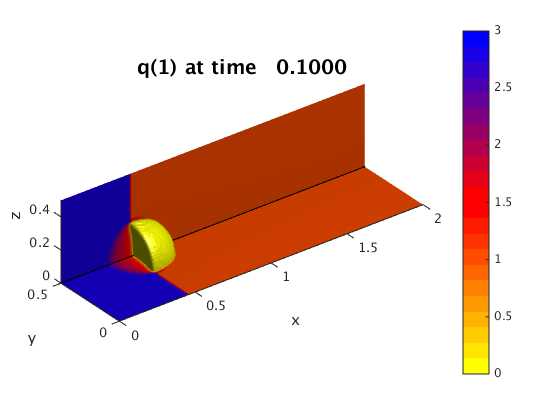
\includegraphics[width=0.45\textwidth]{f1.png}}\hfil
    \plotbox{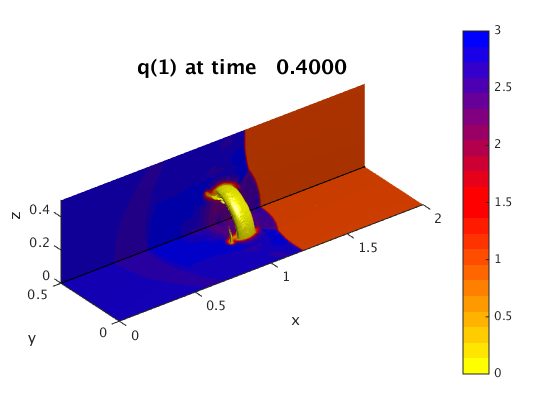
\includegraphics[width=0.45\textwidth]{f4.png}}
  \end{center}
\caption{\amrclaw example demonstrating a
  shock-bubble interaction in the Euler equations of compressible
  gas-dynamics at two times, illustrating the need for adaptive refinement
  to capture localized behavior. The
  $40\times 10\times 10$ grid at Level 1 is refined where needed
  by factors of 4 and then 2 in this 3-level run.}
\label{fig:shockbubble}
\end{figure}

\begin{figure}[h]
  \begin{center}
    % \includegraphics[width=0.45\textwidth]{amr_scaling}
    \plotbox{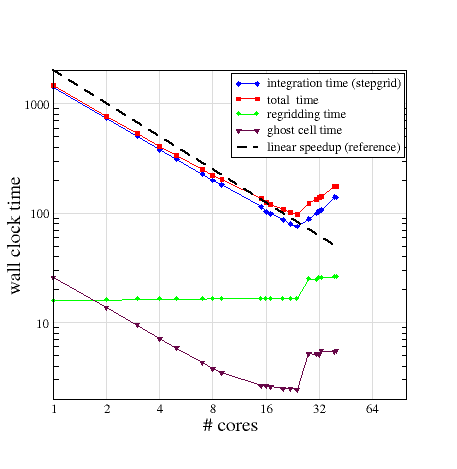
\includegraphics[width=0.4\textwidth,
      clip=true,trim=0cm 1cm 1cm 2cm]{cpuTime.png}}\hfil
    \plotbox{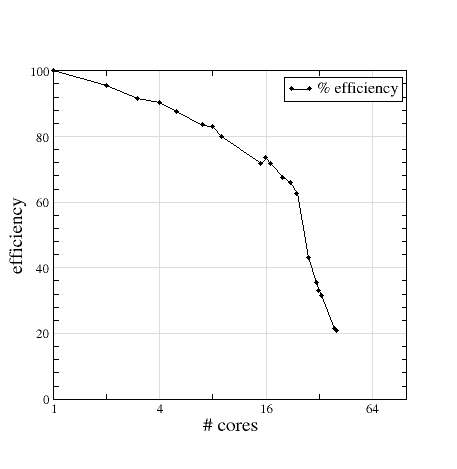
\includegraphics[width=0.4\textwidth,
      clip=true,trim=0cm 1cm 1cm 2cm]{efficiency.png}}
  \end{center}
  \caption{Left is strong scaling results for the \amrclaw example shown in
    \cref{fig:shockbubble}.
    Right is plot of efficiency based on total computational time.}
  \label{fig:amr_scaling}
\end{figure}

The parallelization of \amrclaw and \geoclaw assumes multi-core machines for the
target architecture.  \pyclaw, on the other hand, does not include AMR but uses
MPI via PETSc to achieve parallelism on distributed memory machines that scale
to tens of thousands of cores (see \cref{sec:pyclaw}). Other frameworks exist,
most notably \forestclaw \cite{Burstedde:we}, which are being developed in
parallel with \amrclaw, that provide scalable AMR calculations on large
distributed
memory machines.

%!TEX root = paper.tex
%
% GeoClaw
%
% Lead currently:  Randy LeVeque
%

\subsection{\geoclaw} \textbf{Randy}
\begin{itemize}
    \item NTHMP benchmarks
    \item setaux copying for faster topography integration, recursive 
    \item new topotools and dtopotools
    \item multiple dtopo files
    \item fixed grid monitoring of max values
    \item Spatially varying boundary conditions
\end{itemize}
%!TEX root = paper.tex
%
% PyClaw
%
% Lead currently:  David Ketcheson
%

\subsection{\pyclaw}

Later 4.x releases included a number of Python-based tools for handling
Clawpack input and output.  The 5.0 release includes a full-fledged Python
solver in which the higher-level parts of Clawpack have been reimplemented in
Python.  This new solver also includes access to the high-order algorithms
introduced in SharpClaw and can be used on large distributed-memory parallel
machines.  Lower-level code (whatever gets executed repeatedly and needs to be
fast) from the earlier Fortran Classic and SharpClaw codes is automatically
wrapped at install time using f2py.

\subsubsection{Librarization and extensibility}
Scientific software is easier to use, extend, and integrate with other tools when
it is designed as a library \cite{brown2014run}.  Clawpack has always been designed
to be extensible, but PyClaw takes this further in several ways.  First, it is
distributed via a widely-used package management system, pip.
Second, the default installation process ("pip install clawpack")
provides the user with a fully-compiled code and does not require setting environment
variables.  Like other Clawpack packages, PyClaw provides several "hooks" for users
to plug in custom routines (for instance, to specify boundary conditions).
In PyClaw, these routines -- including the Riemann solver itself -- are selected at
run-time, rather than at compile-time.  These routines can be written directly in
Python, or (if they are performance-critical) in a compiled language (like Fortran or C)
and wrapped with one of the many available tools.  Problem setup (including things like
initial conditions, algorithm selection, and output specification) is also
performed at run-time, which means that researchers can bypass much of the slower
code-compile-execute-postprocess cycle.
It is intended that PyClaw be easily usable within other packages (without control of main()).

\subsubsection{Python classes for data on collections of structured grids}
PyClaw includes Python classes for describing collections of structured grids
and data on them.
These classes are also used by the other codes through VisClaw, for post-processing.

Briefly describe: Dimension, Grid, Patch, State, Solution, Controller.

\subsubsection{PyClaw Solvers}
\begin{itemize}
    \item Classic
    \item SharpClaw: new things include WENO (up to 17th order and in 3D), RK and multistep
            time integration with rigorous SSP timestepping (Yiannis)
\end{itemize}

\subsubsection{PyClaw backends}
\begin{itemize}
    \item pure numpy
    \item PETSc
    \item Boxlib (Matt)
\end{itemize}

\begin{itemize}
    \item overall structure/languages figure
    \item IPython notebooks
\end{itemize}

%!TEX root = paper.tex
%
% VisClaw
%
% Lead currently:  None
%

\newcommand{\cpack}{{\sc ClawPack}\xspace}

\newcommand{\vclaw}{{\sc VisClaw}\xspace}
\newcommand{\aclaw}{{\sc AMRClaw\xspace}\xspace}
\newcommand{\gclaw}{{\sc GeoClaw\xspace}\xspace}
\newcommand{\cclaw}{{\sc Classic Claw}\xspace}
\newcommand{\pclaw}{{\sc PyClaw}\xspace}
\newcommand{\agis}{{\sc ArcGIS}\xspace}
\newcommand{\qgis}{{\sc QGIS}\xspace}

\newcommand{\mlab}{{\sc Matlab}\xspace}
\newcommand{\mplotlib}{{\sc matplotlib}\xspace}
\newcommand{\visit}{{\sc VisIt}\xspace}
% \newcommand{\comment}[1]{\red{#1}}

\subsection{VisClaw : Graphics for visualizing \cpack output}
A practical way to visualize the results of simulations is
essential to any software package focused on solving PDEs.
This is particularly true for simulations making use of adaptive mesh
refinement methods, since most available visualization packages do not
have tools that conveniently visualize hierarchical AMR data.

From its very first release,
\cpack has included tools for visualizing the output of \cpack and
\aclaw runs.  Up until the release of version \cpack 4.x, these
visualization tools consisted primarily of a suite of \mlab routines
for creating custom one, two and three dimensional plots including
pseudo-color plots, Schlieren plots, contour plots and scatter plots
of radially or spherically symmetric data. All of the routines were
specially designed to handle the particular file formats produced by
\cpack and to visualize AMR data.  Built-in tools were also available
for handling one, two and three-dimensional mapped grids.
Starting with version 4.x, however, it was recognized that a reliance
on proprietary software for visualization prevented a sizable
potential user base from making use of the \cpack software.  As a
result, it was decided to convert the one and two dimensional plotting
routines from \mlab to routines written for the \mplotlib,\todo{This
capitalization looks non-standard? It's usually just \texttt{matplotlib}}
a popular open source
Python package for producing publication quality graphics
for one and two dimensional data \cite{Hunter:2007}.

With the development of \cpack Version 5.x, Python graphics tools
have been collected in \vclaw, available as a submodule in the
\cpack GitHub organization.  The \vclaw suite of tools extends the
functionality of the existing 4.x Python routines for creating one and
two dimensional plots, and adds several new capabilities.  Chief among
these new capabilities are the ability to generate output to webpages,
where a series of plots can be viewed individually or as an animated
time sequence using the Javascript package {\sc JSAnimation}
\cite{jsanimation}.
The \vclaw module {\tt iplotclaw} provides
interactive plotting capabilities from the Python or IPython prompt.
Providing much of the same interactive capabilities as the original
\mlab routines, {\tt iplotclaw} allows the user to step,
interactively, through a time sequence of plots, jump from one frame
to another, or interactively explore data from the current time frame.

\vclaw provides support for all of the main \cpack submodules, including
\cclaw, \aclaw, \pclaw and \gclaw.

\subsubsection{Tools for visualizing geo-spatial data produced by \gclaw}
The geo-spatial data generated by \gclaw has particular visualization
requirements.  Tsunami or storm surge simulations are most useful when
the plots showing inundation or flooding levels are overlaid onto
background bathymetry or topography.  Supplementary one dimensional
time series data (e.g. gauge data) numerically interpolated from
the simulation at fixed spatial locations are most useful when
compared graphically to observational data.  Finally, to more
thoroughly analyze the computational data, simulation data
should be made available in formats that can be easily exported to GIS tools
such as \agis or the open source alternative \qgis
\cite{arcgis,qgis}.  For exploration of preliminary results or
communicating results to non-experts, Google
Earth is also helpful.

The latest release of \cpack includes many specialized \vclaw routines
for handling the above issues with plotting geo-spatial data.
Topography or bathymetry data that was
used in the simulation will be read by the graphing routines, and,
using distinct colormaps, both water and land can be viewed on the
same plot.   Additionally, gauge locations can be added, along with contours
of water and land.  One dimensional gauge plots are also created, according to
user-customizable routines. In these gauge plotting routines,
users can easily include  observational data to compare with \gclaw
simulation results.

In addition to HTML and Latex formats (described above), \vclaw will now also
produce KML and KMZ files suitable for visualizing results in Google Earth.
Using the same \mplotlib graphics routines, \vclaw creates PNG files
that can be used as GroundOverlay features in a KML file.  Other features, such
as gauges, borders on AMR grids, and user specified regions can also be
shown on Google Earth.  All KML and PNG files are compressed into a single
KMZ file  that can be opened directly in Google Earth or made available on-line.
While \vclaw does not have any direct support for \agis or \qgis,
the  KML files created for Google Earth can be edited for
export, along with associated PNG files to these other GIS applications.

\subsubsection{Matlab plotting routines}
The \mlab plotting available in early versions of \cpack are also included in
\vclaw.  While most of the one and two dimensional capabilities
available originally in the \mlab suite have been ported to Python and
\mplotlib, the original \mlab routines are still available in the \mlab suite of
plotting tools.  Other plotting capabilities, such as two dimensional
manifolds embedded in three dimensional space, or three dimensional
plots of fully 3d data are only available in the \mlab routines in a way that
interfaces directly with \clawpack.
%via some other package such as \visit \cite{HPV:VisIt}.
More advanced 3d plotting capabilities are planned for future releases of \vclaw.


%!TEX root = paper.tex
%
% Future Work
%
% Lead currently:  None
%

\section{Conclusions} \label{sec:conclusions}

\clawpack has evolved over the past 20 years from its genesis as a small and
focused software package that two core developers could manage without
version control.  It is now an ecosystem of related projects that share a core
philosophy and some common code (notably Riemann solvers and visualization
tools), but that are aimed at different user
communities and that are developed by overlapping but somewhat distinct
groups of developers scattered at many institutions.  The adoption of better
software engineering practices, in particular the use of Git and GitHub as an
open development platform and the use of pull requests to discuss proposed
changes, has been instrumental in facilitating the development of many of the
new capabilities summarized in this paper.  

\subsection{Future Plans} \label{sub:future}

The \clawpack development team continues to look forward to new ideas and
efforts that will allow great accessibility to the project as well as new
capabilities that the core development team has not thought of.  To this end a
number of the broad efforts that are being considered for the next major release
of \clawpack include
\begin{itemize}
    \item An increased librarization effort with the Fortran based sub-packages,
    \item An extensible and more accessible interface to the Riemann solvers,
    \item An effort to allow \pyclaw and the \clawpack Fortran packages to rely
    on more of the same code-base,
    \item An increased emphasis on a larger development community,
    \item More support for new frameworks such as \forestclaw \cite{Burstedde:we},
    \item \revised{Adjoint error estimation for flagging cells to increase
    the efficiency of the AMR codes \cite{DavisLeVeque:adjoint1},}
    \item A refactoring of the visualization tools in \visclaw, along with
    support for additional backends, particularly for three-dimensional results
    (e.g.
\revised{
\texttt{Mayavi}\footnote{\url{http://docs.enthought.com/mayavi/mayavi/}},} 
\texttt{VisIt}\footnote{\url{https://visit.llnl.gov}}, 
\texttt{ParaView}\footnote{\url{http://www.paraview.org/}}, or 
\texttt{yt}\footnote{\url{http://yt-project.org/}}).
\end{itemize}

\section*{Acknowledgements}
\revised{
Clawpack development has been funded by many agencies and institutions over
the past 20 years.  The improvements
cataloged in this paper have been funded in part by
DOE grant DE-FG02-88ER25053, NSF grants DMS-1216732, EAR-1331412,
The latest developments have also built on the work of many earlier Clawpack
developers and users, many of whom are acknowledged on the Clawpack Authors
webpage.
}



\bibliographystyle{siamplain}
\bibliography{paper}

\end{document}
